% !TEX root = main.tex
\section{Auswertung Milchstrasse}
\begin{figure}[H]
    \centering
    \input{plots/Belichtungszeit.tex}   
    \caption[Gemessenen Spektren bei verschiedenen Belichtungszeiten]{Mithilfe dieser Abbildung lässt sich erkennen wie sich die gemessenen Spektren mit der Belichtungszeit verändern. Bei einer Belichtungszeit von \SI{1}{s} ist ein sehr ausgeprägtes Rauschen des Signals zu verzeichnen. Maxima sind bei dieser Belichtungszeit kaum ausmachbar. Das Rauschen ist allerdings schon bei einer Belichtungszeit von \SI{10}{s} deutlich reduziert ausgeprägt. Maxima lassen sich bei dieser Belichtungszeit deutlich genauer ausmachen.}
    \label{fig:Belichtungszeit}
\end{figure}

\begin{figure}[H]
    \centering
    \input{plots/BelichtungszeitExtrema.tex}   
    \caption[Eindeutigen Unterschiede der Spektren bei verschiedenen Belichtungszeiten]{Diese Abbildung soll noch einmal die eindeutigen Unterschiede der Spektren bei verschiedenen Belichtungszeiten verdeutlichen. Da sich das Spektrum bei einer Belichtungszeit von \SI{30}{s} und \SI{300}{s} nur noch minimal unterscheidet. Haben wir eine Belichtungszeit für unsere Spektren von \SI{60}{s} gewählt. Bei dieser Zeit sind alle Maxima deutlich ausmachbar und der zeitlich begrenzte Versuchszeitraum wird nicht gesprengt.}
    \label{fig:BelichtungszeitExtremal}
\end{figure}

\begin{figure}[H]
    \centering
    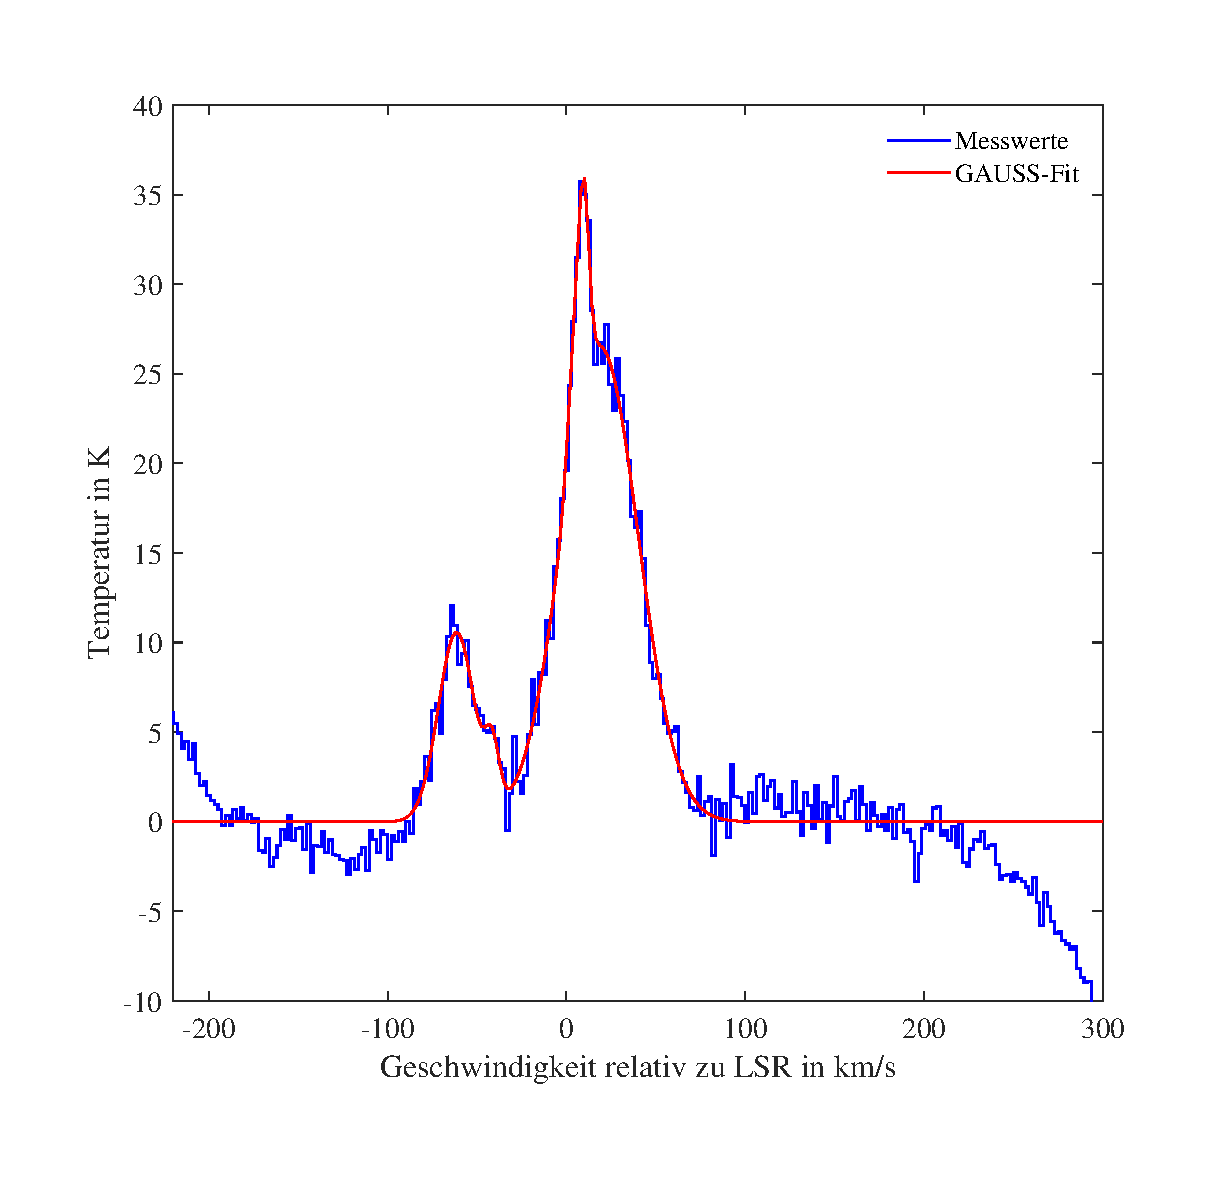
\includegraphics[width= 0.9\textwidth]{plots/TestBaseline.eps}
    \caption[Gemessenes Beispielspektrum zur Darstellung der Verarbeitung der Daten]{Gemessenes Beispielspektrum zur Darstellung der Verarbeitung der Daten. Da bei den Messungen stets ein Untergrundrauschen mitgemessen wird, muss dieses mithilfe eines Computerprogramms herausgefiltert werden. Mithilfe eines MatLab-Skripts sind die Spektren jeweils noch mit Gaußfunktionen gefittet. So lassen sich die Maxima deutlich erkennen und auslesen. In diesem Fall handelt es sich um eine Messung bei $l = \SI{30}{\degree}, \, b = \SI{0}{\degree}$ und die beiden Maxima liegen bei \SI{7.3}{\frac{km}{s}} und \SI{-64.8}{\frac{km}{s}} relativ zu LSR.}
    \label{fig:TestBaseline}
\end{figure}

\begin{figure}[H]
    \centering
    \input{plots/VvonR.tex}
    \caption[Rotationskurve der Milchstraße]{Dargestellt ist eine Rotationskurve der Milchstraße. Die eingetragenen Datenpunkte sind jeweils aus dem Peak der maximal verschobenen Geschwindigkeitskomponente der gemessenen Geschwindigkeitsspekra aus dem ersten Quadranten gewonnen. Es ist deutlich zu erkennen, dass die Geschwindigkeit $V(R)$ nahezu unabhängig von dem Bahnradius ist. Mit einem linearen fit ist dies in der Abbildung nochmals verdeutlicht. Der Ordinatenabschnitt kennzeichnet dabei den Mittelwert der gemessenen Geschwindigkeiten. Dieser beträgt $\SI{210.9 \pm 3.1}{\frac{km}{s}}$ und kommt dem einem Literaturwert von $\SI{220}{\frac{km}{s}}$ \cite{LSR} sehr nahe. Einen exakten Literaturwert für die Geschwindigkeit zu finden ist nicht möglich, da dieser bei verschiedenen Quellen unterschiedlich angegeben wird. Jedoch wird immer ein Wert um $\SI{220}{\frac{km}{s}}$ angegeben.}
    \label{fig:VvonR}
\end{figure}
Da es im ersten Quadranten mehrere positive Lösungen für $r$ gibt, muss eine genauere Untersuchung der Beobachtungsrichtung gemacht werden. Hierfür werden
\begin{figure}[H]
    \centering
    \input{plots/bungleichnull.tex}   
    \caption[Spektren für verschiedene galaktische Breiten $b$]{Spektren für verschiedene galaktische Breiten $b$. Erkennbar ist, dass bei den Spektren stets bei allen gewählten galaktische Breiten $b$ die Maxima bei \SI{2.4}{\frac{km}{s}}, \SI{-30.6}{\frac{km}{s}} und bei \SI{-69.7}{\frac{km}{s}} erkennbar sind. Die gewählten galaktischen Breiten sind also zu klein gewählt worden. Bei größeren galaktischen Breiten sollte dann mindestens ein Peak verschwinden. Auf die gefitteten Gaußkurven wurde bei dieser Abbildung aus Gründen der Lesbarkeit verzichtet.}
    \label{fig:bungleichnull}
\end{figure}

\begin{figure}[H]
    \centering
    \input{plots/Milchstrassesafe.tex}   
    \caption[Abbildung der Milchstraße]{In dieser Abbildung ist die Milchstraße mithilfe der Daten aus den Frequenzspektra katografiert. Bei der Abbildung ist ein Seitenarme der Milchstraße im Bereich um $(x,y)=(10,-10)$ deutlich ersichtlich. Ein weiterer Galaxiearm ist im Bereich $(x,y)=(10,5)$ erkennbar, wobei dieser schon deutlich schwächer ausgeprägt ist. In dem Bereich um den Ursprung sind die Datenpunkte sehr dicht angehäuft. Somit ist in diesem Bereich leider keine eindeutige Aussage über etwaige Galaxiearme treffbar. Mithilfe des eingefärbten Kreises mit dem Radius von $\si{25}{kpc}$ ist die größe der gesamten Galxie ersichtlich.}
    \label{fig:Milchstrassesafe}
\end{figure}



